% Title: gl2ps_renderer figure
% Creator: GL2PS 1.4.2, (C) 1999-2020 C. Geuzaine
% For: Octave
% CreationDate: Wed Oct 19 08:50:18 2022
\setlength{\unitlength}{1pt}
\begin{picture}(0,0)
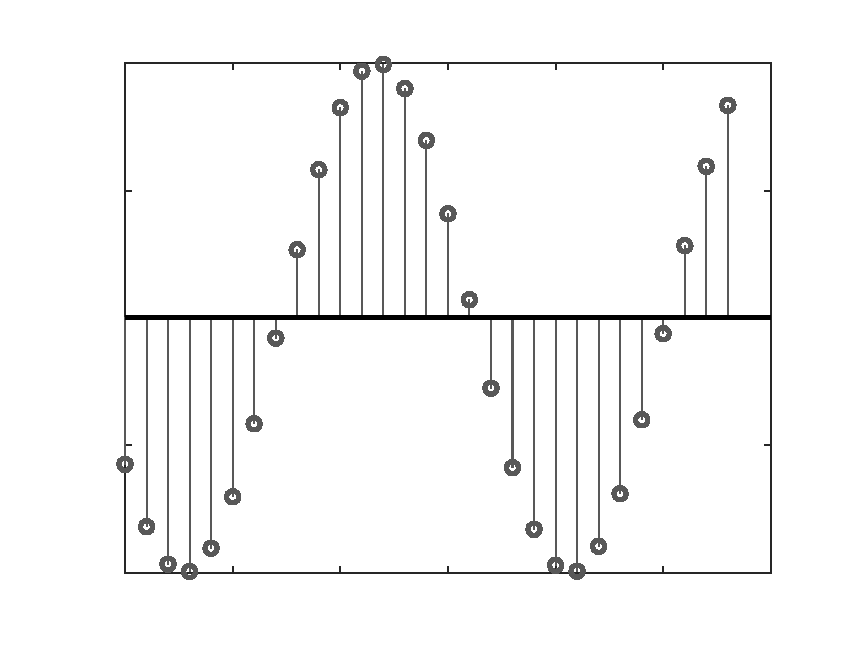
\includegraphics[scale=1]{octaves/stem-plot-inc}
\end{picture}%
\begin{picture}(400,300)(0,0)
\fontsize{6}{0}\selectfont\put(52,27.8){\makebox(0,0)[t]{\textcolor[rgb]{0.15,0.15,0.15}{{-10}}}}
\fontsize{6}{0}\selectfont\put(103.667,27.8){\makebox(0,0)[t]{\textcolor[rgb]{0.15,0.15,0.15}{{-5}}}}
\fontsize{6}{0}\selectfont\put(155.333,27.8){\makebox(0,0)[t]{\textcolor[rgb]{0.15,0.15,0.15}{{0}}}}
\fontsize{6}{0}\selectfont\put(207,27.8){\makebox(0,0)[t]{\textcolor[rgb]{0.15,0.15,0.15}{{5}}}}
\fontsize{6}{0}\selectfont\put(258.667,27.8){\makebox(0,0)[t]{\textcolor[rgb]{0.15,0.15,0.15}{{10}}}}
\fontsize{6}{0}\selectfont\put(310.333,27.8){\makebox(0,0)[t]{\textcolor[rgb]{0.15,0.15,0.15}{{15}}}}
\fontsize{6}{0}\selectfont\put(362,27.8){\makebox(0,0)[t]{\textcolor[rgb]{0.15,0.15,0.15}{{20}}}}
\fontsize{6}{0}\selectfont\put(48.5263,33){\makebox(0,0)[r]{\textcolor[rgb]{0.15,0.15,0.15}{{-1}}}}
\fontsize{6}{0}\selectfont\put(48.5263,94.125){\makebox(0,0)[r]{\textcolor[rgb]{0.15,0.15,0.15}{{-0.5}}}}
\fontsize{6}{0}\selectfont\put(48.5263,155.25){\makebox(0,0)[r]{\textcolor[rgb]{0.15,0.15,0.15}{{0}}}}
\fontsize{6}{0}\selectfont\put(48.5263,216.375){\makebox(0,0)[r]{\textcolor[rgb]{0.15,0.15,0.15}{{0.5}}}}
\fontsize{6}{0}\selectfont\put(48.5263,277.5){\makebox(0,0)[r]{\textcolor[rgb]{0.15,0.15,0.15}{{1}}}}
\fontsize{7}{0}\selectfont\put(207,287.5){\makebox(0,0)[b]{\textcolor[rgb]{0,0,0}{{A stem plot of a sinusoidal sequence}}}}
\end{picture}
